\chapter{Применение метода М-последовательности к экспериментальному исследованию дифракционных задач}

В данной главе описывается применение метода MLS к акустическому дифракционному эксперименту. Предлагается метод вычисления части импульсного отклика, не относящейся к излучающему и приемному трактам, а относящейся исключительно к дифракционному процессу. Используется измерение объемной скорости с помощью метода двух микрофонов, открытый конец источника моделируется с помощью поправки Вайнштейна \cite{Weinstein1966}. В последующих главах данная методика применяется для различных акустических дифракционных экспериментов.

\section{Последовательность максимальной длины}

Последовательность максимальной длины (Maximum Length Sequence, MLS) представляет собой псевдослучайную периодическую двоичную последовательность, автокорреляционная функция которой очень близка к периодически повторяющемуся единичному импульсу. Последовательность $\{ S_k = \pm 1 \}$ порядка $M$ имеет период $L = 2^M - 1$, а ее автокорреляционная функция $\{ A_k\}$ имеет вид:

\begin{equation}
A_k = \frac{1}{L} \sum_{n=1}^{L} S_n S_{n+k-1} = 
\begin{cases}
1, & k = 1;\\
-1/L, & k=2\dots L.
\end{cases}
\end{equation}

Благодаря этому свойству MLS, ее можно использовать для измерения импульсного отклика линейных стационарных систем. Если подать на вход системы сигнал в виде М-последовательности и вычислить взаимнокорреляционную функцию выходного сигнала с М-последовательностью, получится сигнал, представляющий собой отклик системы на автокорреляционную функцию М-последовательности - практически отклик на дельта-функцию, то есть сигнал, близкий к импульсному отклику системы.

Действительно, пусть $\{R_k \}$ — отклик системы на М-последовательность  $\{S_k \}$, а  $\{G_k \}$ — импульсный отклик системы. Тогда  $\{R_k \}$ есть свертка  $\{S_k \}$ и  $\{G_k \}$:

\begin{equation}
R_k = \sum_{n=1}^{L} S_{k-n} G_n,
\end{equation}
а взаимная корреляция  $\{H_k \}$ последовательностей  $\{R_k \}$ и  $\{S_k \}$ есть отклик системы на  $\{A_k \}$:

\begin{equation}
H_k = \frac{1}{L} \sum_{m=1}^{L} S_m R_{k+m} = \frac{1}{L} \sum_{m=1}^{L} S_m \sum_{n=1}^{L} S_{k+m-n} G_n = \sum_{n=1}^{L} A_{k-n} G_n \approx G_k.
\end{equation}

\section{Схема эксперимента}

Общая схема эксперимента представлена на (Рис. \ref{img:ris0_1}). На вход системы подается М-последовательность $\{ S_k^{\text{in}}\}$ . Этот сигнал через ЦАП и усилитель подается на источник акустических волн. Микрофон располагается вблизи рассеивателя или на его поверхности. Сигнал с микрофона усиливается и преобразуется в цифровой вид. После этого вычисляется взаимнокорреляционная функция $\{ H_k^{\text{in}}\}$ выходного и входного сигналов:

\begin{equation}
H_k = \frac{1}{L} \sum_{n=1}^{L} S_n^{\text{in}} S_{k+n}^{\text{out}}.
\end{equation}

\begin{figure}[ht]
	\centering
	\includegraphics [scale=0.8] {ris0_1}
	\caption{Схема эксперимента.}
	\label{img:ris0_1}
\end{figure}

Следует отметить, что для такой постановки эксперимента не требуется использовать безэховые помещения, поскольку полезный сигнал от рассеивателя появляется в импульсном отклике системы раньше помех, приходящих от акустического окружения. Для надежного разделения полезного и паразитного сигналов следует располагать рассеиватель на достаточном удалении от пола и прочих предметов, а затем применять окно во временной области, отсекая паразитные сигналы. Сигнал $\{ H_k \}$ — отклик системы на $\{ A_k \}$. Он близок к импульсному отклику всей системы и включает в себя, помимо чисто волновой части, еще и отклики источника и электрических трактов. Вопрос выделения из него полезной части рассматривается ниже.


\section{Оборудование и параметры эксперимента}

В данной работе в качестве входного сигнала использовалась М-последовательность порядка $M = 19$. Частота дискретизации ЦАП и АЦП составляла $F_s = 48000$ Гц. Такие параметры дают длительность входного сигнала $T = (2^M - 1)/F_s \approx 4$ с. Источником служил Bruel\&Kjaer 4295 OmniSource с адаптером, позволяющим измерять объемную скорость источника (4299 Volume Velocity Adaptor). Схема источника с адаптером приведена на (Рис. \ref{img:ris0_2}).

\begin{figure}[ht]
	\centering
	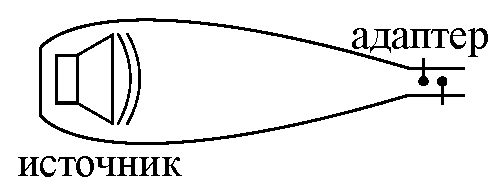
\includegraphics [scale=1] {ris0_2}
	\caption{Схема источника с адаптером для измерения объемной скорости.}
	\label{img:ris0_2}
\end{figure}

Источник представляет собой электродинамическую головку, помещенную в продолговатый пластиковый корпус с узким отверстием (3,75 см). Такая конструкция позволяет создавать акустическое поле, близкое к полю точечного монопольного источника. Адаптер представляет собой пластиковую трубку кругового сечения, плотно пригнанную к выходному отверстию источника. Внутрь трубки помещены два микрофона, сигналы с которых используются для восстановления объемной скорости источника. Для регистрации рассеянного сигнала использовался Bruel\&Kjaer 4957 1/4 inch Array Microphone, характеристики которого близки к характеристикам микрофонов в адаптере.

\section{Выделение импульсного отклика, связанного только с дифракционным процессом}

Как уже было сказано, сигнал $\{ H_k \}$ необходимо очистить, выделив импульсный отклик дифракционного процесса. Заметим, что основные помехи вносятся источником звука OmniSource, в котором происходят многочисленные
переотражения.

Для простоты будем рассматривать дискретные сигналы $\{ A_k \}$ и $\{ H_k \}$ как непрерывные сигналы $A(t)$ и $H(t)$. При этом будем помнить, что Фурье-образы таких сигналов определены для дискретного набора частот. Введем следующие функции:

\begin{enumerate}
	\item $W(t)$ - производная объемной скорости источника по времени при подаче на вход системы сигнала $A(t)$.
	\item $H^{\text{prop}}(t)$ - импульсный отклик, описывающий распространение волны от источника до микрофона (именно он нас и интересует), определяемый соотношением
	\begin{equation}
	p(t) = \frac{\rho_0}{4\pi} \int_{-\infty}^{\infty} W(\tau) H^{\text{prop}}(t-\tau) d\tau,
	\end{equation}
	где $p(t)$ - давление в точке наблюдения при подаче на вход системы сигнала $A(t)$, $\rho_0$ - плотность воздуха.
	\item $H^{\text{recv}}(t)$ - импульсный отклик приемной части (микрофона, усилителя и АЦП), определяемый соотношением
	\begin{equation}
	H(t) = \int_{-\infty}^{\infty} p(\tau) H^{\text{recv}}(t-\tau)d\tau
	\end{equation}
\end{enumerate}

Нормировочный множитель $\rho_0/4\pi$ в формуле, определяющей $H^{\text{prop}}$, введен из следующих соображений. Хорошо известно, что в свободном пространстве точечный монопольный источник создает давление, пропорциональное производной его объемной скорости по времени:

\begin{equation}
p = \frac{\rho_0}{4\pi R} W(t-R/c),
\end{equation}
где $R$ - расстояние от источника до точки наблюдения. Таким образом, в этом случае импульсный отклик $H^{prop}$ представляет собой дельта-функцию (в дискретном случае — одиночный импульс):
\begin{equation}
H^{\text{prop}} = \frac{\delta(t-R/c)}{R}.
\end{equation}

Амплитуда дельта-функции обратно пропорциональна расстоянию до источника $R$ и обращается в единицу при $R = 1$ м, что удобно.
Будем обозначать Фурье-образ сигнала $\zeta(t)$ как $\zeta_\omega$. Тогда для наших сигналов будем иметь:

\begin{eqnarray}
&p_\omega = W_\omega H_\omega^{\text{prop}},\\
&H_\omega = p_\omega H_\omega^{\text{recv}}.
\end{eqnarray}
Если удастся измерить производную по времени объемной скорости источника $W(t)$, то можно будет восстановить дифракционную часть импульсного отклика:

\begin{equation}
\label{eq:mls_main}
H_\omega^{\text{prop}} = \frac{H_\omega}{W_\omega H_\omega^{recv}}.
\end{equation}

Заметим, что предложенная процедура выделения части импульсного отклика, связанной только с дифракционным процессом никак не использует преимуществ метода М-последовательностей. Действительно, и $W_\omega$ и $H_\omega$ пропорциональны спектру входного сигнала, а значит, при любом достаточно широкополосном входном сигнале ~\eqref{eq:mls_main} дает возможность восстановить функцию $H^{\text{prop}}(t)$. Тем не менее, использование М-последовательностей позволяет повысить качество восстановления.

Длительность используемого в эксперименте сигнала \textbf{(4 с)} соответствует более чем 1 км пути, проходимого волной. При этом нас интересуют только первые несколько метров импульсного отклика, а вся остальная его часть является помехой. Чтобы ослабить влияние этой помехи, используем для вычисления Фурье-образов только начальную часть сигналов $H(t)$ и $W(t)$. Длительность этой части следует взять такой, чтобы в нее попала вся существенно ненулевая часть сигнала $W(t)$. В описываемых ниже экспериментах использовались первые 50 м сигналов $H(t)$ и $W(t)$, что соответствует примерно 100 переотражениям в корпусе источника.

\section{Измерение производной объемной скорости источника}

Как было сказано ранее, для измерения объемной скорости источника может быть применен адаптер с двумя микрофонами. Схема используемого адаптера приведена на (Рис. \ref{img:ris0_3}).

\begin{figure}[ht]
	\centering
	\includegraphics [scale=1.2] {ris0_3}
	\caption{Схема адаптера для измерения объемной скорости источника.}
	\label{img:ris0_3}
\end{figure}

Пусть при подаче на вход системы М-последовательности $\{ S_k^{\text{in}} \}$ с микрофонов адаптера после усиления и ЦАП приходят сигналы $\{ S_k^{\text{out, 1}} \}$ и $\{ S_k^{\text{out, 2}} \}$. Пусть $\{ H_k^{\text{1, 2}} \}$ — взаимные корреляции этих сигналов с входным сигналом $\{ S_k^{\text{in}} \}$. Обозначим через $p_{1,2}$ начальные части (первые 50 м) сигналов $H^{1,2}$.

Для вычисления объемной скорости предположим, что внутри адаптера распространяются только поршневые моды. Обоснованность этого предположения обсуждается ниже. При таком предположении для каждой частоты $\omega$ давление в трубке может быть представлено в следующем виде:
\begin{equation}
p_\omega(x) = A^{-ikx} + Be^{ikx},
\end{equation}
где $A$ и $B$ — амплитуды волн, распространяющихся в положительном и отрицательном направлении оси $x$ соответственно. Здесь предполагается гармоническая зависимость от времени вида $e^{i\omega t}$. Измеряются давления $p_1(t)$ и $p_2(t)$ в точках $x = -b$ и $x = -a$ соответственно. Для их Фурье-образов можно записать:

\begin{eqnarray}
\label{eq:twomic}
&p_{1\omega} = A e^{ikb} + Be^{-ikb},\\
&p_{2\omega} = A e^{ika} + Be^{-ika},
\end{eqnarray}
откуда:

\begin{equation}
A = \frac{-p_{1\omega}e^{ikb} + p_{2\omega}e^{ika} }{e^{2ika} - e^{2ikb}}, \quad B = \frac{-p_{1\omega}e^{ik(2a+b)} - p_{2\omega}e^{ik(a+2b)} }{e^{2ika} - e^{2ikb}}.
\end{equation}

Пользуясь уравнением Эйлера, для производной колебательной скорости $v$ получим:

\begin{equation}
\label{eq:eq1_16}
\left(\frac{dv}{dt}\right)_\omega = \frac{ik}{\rho_0} (A e^{-ikx} - Be^{ikx}).
\end{equation}

Для производной по времени объемной скорости источника имеем:

\begin{equation}
\label{eq:proizv_vrem}
W_\omega = i\omega \frac{\pi r^2}{\rho_0 c}(A-B),
\end{equation}
где $r$ — радиус трубки адаптера. Полученная формула дает относительно неплохие результаты, однако вносит заметные фазовые искажения. Причиной этих искажений служит то, что трубка не является достаточно тонкой, а значит, ее конец нельзя считать точечным источником. Используя теорию Вайнштейна об излучении волн из открытого конца волновода \cite{Weinstein1966}, можно получить формулу, подходящую для данного случая. Для этого в ~\eqref{eq:eq1_16} надо заменить $B$ на $-A$, то есть

\begin{equation}
W_\omega = i\omega\frac{2\pi r^2 A}{\rho_0 c}.
\end{equation}

Вычисленная таким образом объемная скорость будет содержать в себе также АЧХ приемных трактов адаптера. В действительности микрофоны в адаптере близки по своим характеристикам к микрофону, используемому для регистрации поля вблизи рассеивателя, а АЧХ усилителей в приемных трактах близки к идеальным в интересующем нас диапазоне частот (можно
считать, что $H_\omega^{\text{recv}} = 1$). Формула ~\eqref{eq:mls_main} может быть переписана следующим образом:

\begin{equation}
H_\omega = W_\omega H_\omega^{\text{prop}}.
\end{equation}

Рассмотрим ограничения предлагаемого метода. Очевидной трудностью является то, что формулы \label{eq:twomic} имеют смысл только для частот $f < f_c$, где граничная частота $f_c$ определяется расстоянием между микрофонами: $f_c = c_0/(2(b-a))$. Это частота, при которой знаменатель в \label{eq:twomic} обращается в нуль. В нашем случае \textbf{$f_c = 8.57$} кГц. Таким образом, все сигналы при обработке должны быть пропущены через ФНЧ. 

Другие трудности связаны с модами высших порядков, распространяющимися в трубке адаптера. Эти моды могут влиять на результат двумя способами. Во-первых, они могут излучать звук вовне. Во-вторых, они могут создавать сигнал на микрофонах адаптера, внося ошибки в измерение объемной скорости. Моды высших порядков имеют следующую структуру:

\begin{equation}
p(x, \xi, \varphi) = \exp\{\pm i \gamma x \}\begin{Bmatrix}
\sin(n\varphi) \\
\cos(n\varphi) \\
\end{Bmatrix} J_n(k_{m,n}\xi),
\end{equation}
где $(x, \xi, \varphi)$ — цилиндрические координаты с осью, совпадающей с осью трубки адаптера, $J_n$ — функции Бесселя, $k_{m,n}$ — корни уравнения $J'_n(k_{m,n} r) = 0$, а $\gamma = \sqrt{\omega^2/c_0^2 - k_{m,n}^2}$. Если точка наблюдения расположена вблизи оси системы, что соответствует нашему случаю, то, в силу ортогональности, моды высших порядков не будут давать вклада в излучаемое поле. Все моды, кроме поршневой, имеют свои частоты отсечки, что позволяет оценить их постоянные затухания. Моды с номером $n\neq 0$ не будут влиять на сигналы микрофонов адаптера, поскольку микрофоны расположены на оси трубки, $J_n(0) = 0$ при $n \neq 0$. Поэтому наиболее «опасной»модой будет мода с $J_0(k_{1,0}\xi)$. Простой анализ показывает, что частота отсечки этой моды близкак 11.1 кГц. Для частоты сигнала 5 кГц это соответствует чисто мнимому значению $\gamma = 180i$ $\text{м}^{-1}$. При такой постоянной распространения волна быстро затухает. Таким образом, для частот ниже 5 кГц моды высших порядков можно не рассматривать.

\section{Фильтрация}

Все представленные ниже дифракционные импульсные отклики подвергались фильтрации. Использовалась комбинация фильтров высоких и низких частот со следующими частотными характеристиками. Для ФНЧ:

\begin{equation}
K_{LPF}(f) = \frac{K_0}{2} \left[1 - \text{th} \left(\frac{|f| - f_0}{\Delta f}\right)\right];
\end{equation}

Для ФВЧ:

\begin{equation}
K_{HPF}(f) = K_0 - K_{LPF}(f).
\end{equation}

При этом для фильтра низких частот параметры $f_0$ и $\Delta f$ имели значения $f_0 = 4000$ Гц, $\Delta f$ = 1000 Гц, 
а для фильтра высоких частот $f_0 = 50$ Гц, $\Delta f = 10$ Гц. Нормировочный коэффициент $K_0$ выбирался таким образом, чтобы значение импульсной характеристики результирующего фильтра в нуле было единицей. 

Импульсная характеристика фильтра представлена на Рис. \ref{img:ris0_4}.

\section{Измерения в пустом полупространстве}

Простейшим акустическим окружением, легко реализуемым в эксперименте, является пустое полупространство с жесткой границей. Давление в точке наблюдения в этом случае создается прямой полной и волной, отраженной
от границы полупространства. Импульсный отклик $H^{\text{prop}}$ имеет вид

\begin{equation}
\label{eq:hprop}
H^{\text{prop}} = \frac{\delta(t - R/c)}{R} + \frac{\delta(t - \bar{R}/c)}{\bar{R}},
\end{equation}
где $R$ и $\bar{R}$ — расстояния от точки наблюдения до источника и до отражения источника в границе полупространства соответственно. 

\begin{figure}[ht]
	\centering
	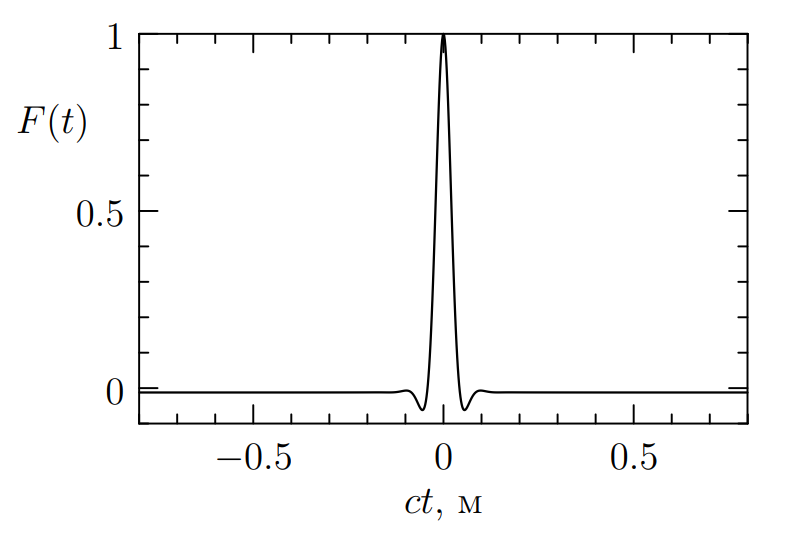
\includegraphics [scale=0.6] {ris0_4}
	\caption{Импульсная характеристика используемого фильтра.}
	\label{img:ris0_4}
\end{figure}

Для проверки работоспособности методики был проведен эксперимент, схема которого показана на (Рис. \ref{img:ris0_5}).

\begin{figure}[ht]
	\centering
	\includegraphics [scale=0.7] {ris0_5}
	\caption{Схема измерений в пустом полупространстве.}
	\label{img:ris0_5}
\end{figure}

Все окружающие предметы были удалены на такое расстояние, чтобы отраженные от них волны приходили на микрофон позже прямой и отраженной от пола волн. Указанное на (Рис. \ref{img:ris0_5}) расположение источника и микрофона соответствует значениям $R = 1$ м и $\bar{R} \approx 4.5$ м. 

В соответствии с ~\eqref{eq:hprop} в импульсном отклике мы должны увидеть две копии импульсной характеристики использованного фильтра (Рис. \ref{img:ris0_4}), сдвинутые в положения $ct = 1$ м и $ct = 4.5$ м. При этом амплитуда первого пика должна быть равна единице, а второго $1/4.5 \approx 0.22$. На (Рис. \ref{img:ris0_6}) показан наблюдаемый в эксперименте импульсный отклик пустого полупространства.

\begin{figure}[ht]
	\centering
	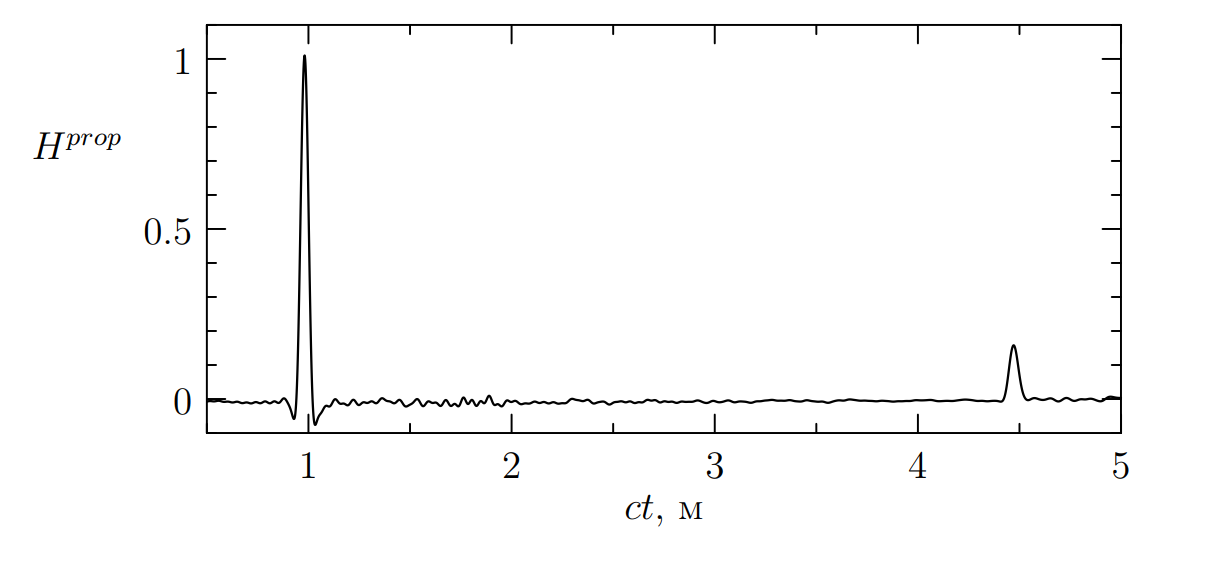
\includegraphics [scale=0.55] {ris0_6}
	\caption{Измеренный импульсный отклик пустого полупространства.}
	\label{img:ris0_6}
\end{figure}

Хорошо видно, что пики имеют правильные положения и что высота первого пика также верна. Высота второго пика несколько ниже предсказанной теоретически, что, по видимому, объясняется неравномерностью диаграммы
направленности использованного источника.

Для иллюстрации роли всех этапов обработки сигнала рассмотрим показанный на (Рис. \ref{img:ris0_7}) импульсный отклик $H^{\text{prop}}$, восстановленный без использования вайнштейновской поправки ~\eqref{eq:proizv_vrem} и импульсный отклик всей системы $H$ (Рис. \ref{img:ris0_8}).

\begin{figure}[ht]
	\centering
	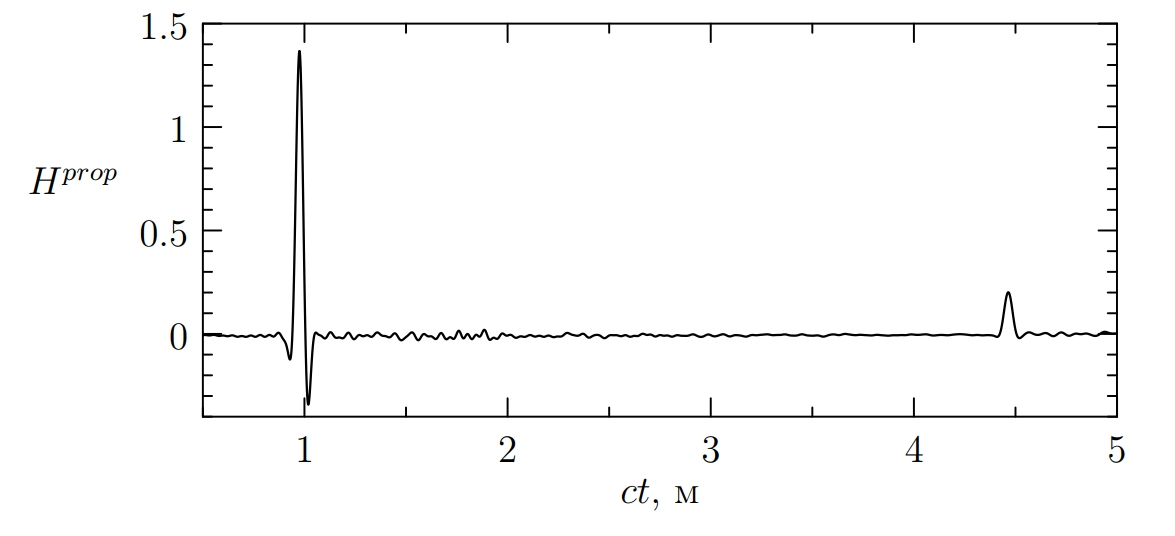
\includegraphics [scale=0.55] {ris0_7}
	\caption{Отклик, восстановленный без использования вайнштейновской поправки.}
	\label{img:ris0_7}
\end{figure}

\begin{figure}[ht]
	\centering
	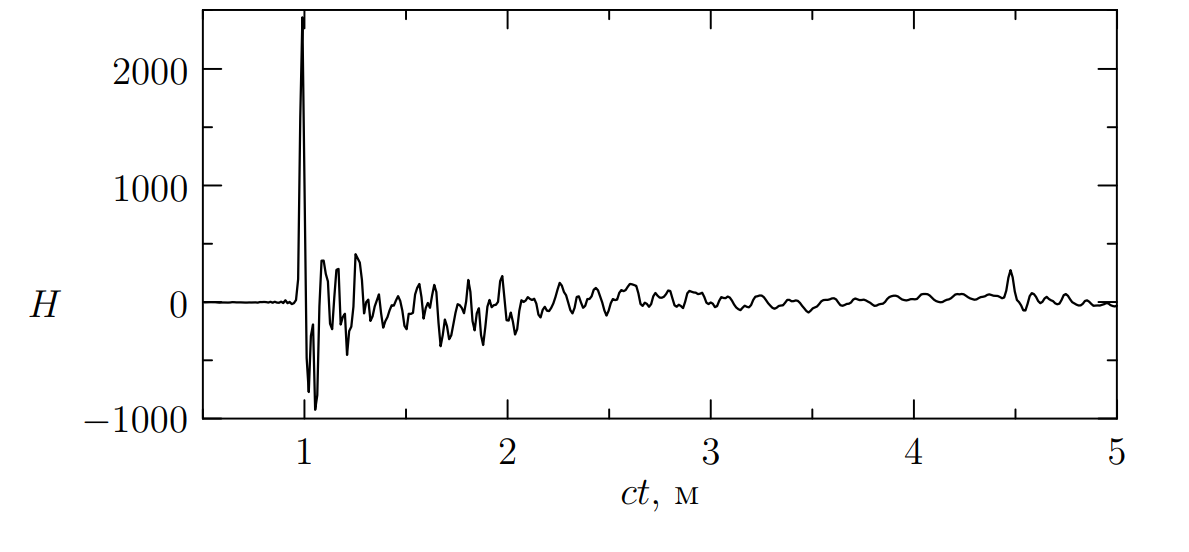
\includegraphics [scale=0.55] {ris0_8}
	\caption{Импульсный отклик всей системы при измерении в пустом полупространстве.}
	\label{img:ris0_8}
\end{figure}

Хорошо видно, что без использования вайнштейновской поправки в восстанавливаемый импульсный отклик вносятся заметные амплитудные и фазовые искажения. В полном импульсном отклике $H$ видны многократные переотражения
внутри источника, делающие сигнал непригодным для анализа.